
\section{Bonus item : ``Real-Time''}

Our additional item is a close attention to the computation time of deblurring.
We develop different techniques to reduce this time and fix as objective around 1 second by picture's deblurring.

The first point is naturally to pay attention to the implementation of our different algorithms. We try to reduce the number of nested loop, even if with color image, and image in general, loops are quite unavoidable.

\todo{Merge from here}
The second point is to crop the image when the whole one is unnecessary. Indeed, for the angle and length estimation of the PSF, we only need a relatively small part of a big picture and we  use the whole image for small pictures. After several tests, we conclude that a $256 \times 256 $ matrix is relevant (i.e. $\pm 1$ degree and $\pm 3$ pixels) for most of the blur and the computation time is then maximum 0.7 second for the angle estimator and maximum 0.05 second for the length estimator, regardless the size of the initial picture. For example the figure \ref{fig:SagarShort} is computed with our crop and needs $0.684 $ [s] and $0.0463$ [s] for the angle and the length respectively whereas the figure \ref{fig:SagarLong} is computed with the whole figure and needs $11.42$ [s] and $1.128$ [s]. So the difference of time is quite big while the difference of quality is acceptable. 

\todo{to here}
The second point is to crop the image when the whole one is unnecessary. Indeed, for the angle and length estimation of the PSF, we only need a relatively small part of a big picture and we  use the whole image for small pictures. After several tests, we conclude that a $256 \times 256 $ matrix is relevant (i.e. $\pm 1$ degree and $\pm 3$ pixels) for most of the blur and the computation time is then around maximum 0.7 second for the angle estimator and maximum 0.05 second for the length estimator, regardless the size of the initial picture. For example the figure \ref{fig:SagarShort} is computed with our crop and needs $0.684 $ [s] and $0.0463$ [s] for the angle and the length respectively whereas the figure \ref{fig:SagarLong} is computed with the whole figure and needs $11.42$ [s] and $1.128$ [s]. So the difference of time is quite big while the difference of quality is acceptable.
\todo{with here}
\begin{figure}[h]
\centering
\begin{subfigure}{0.4\textwidth}
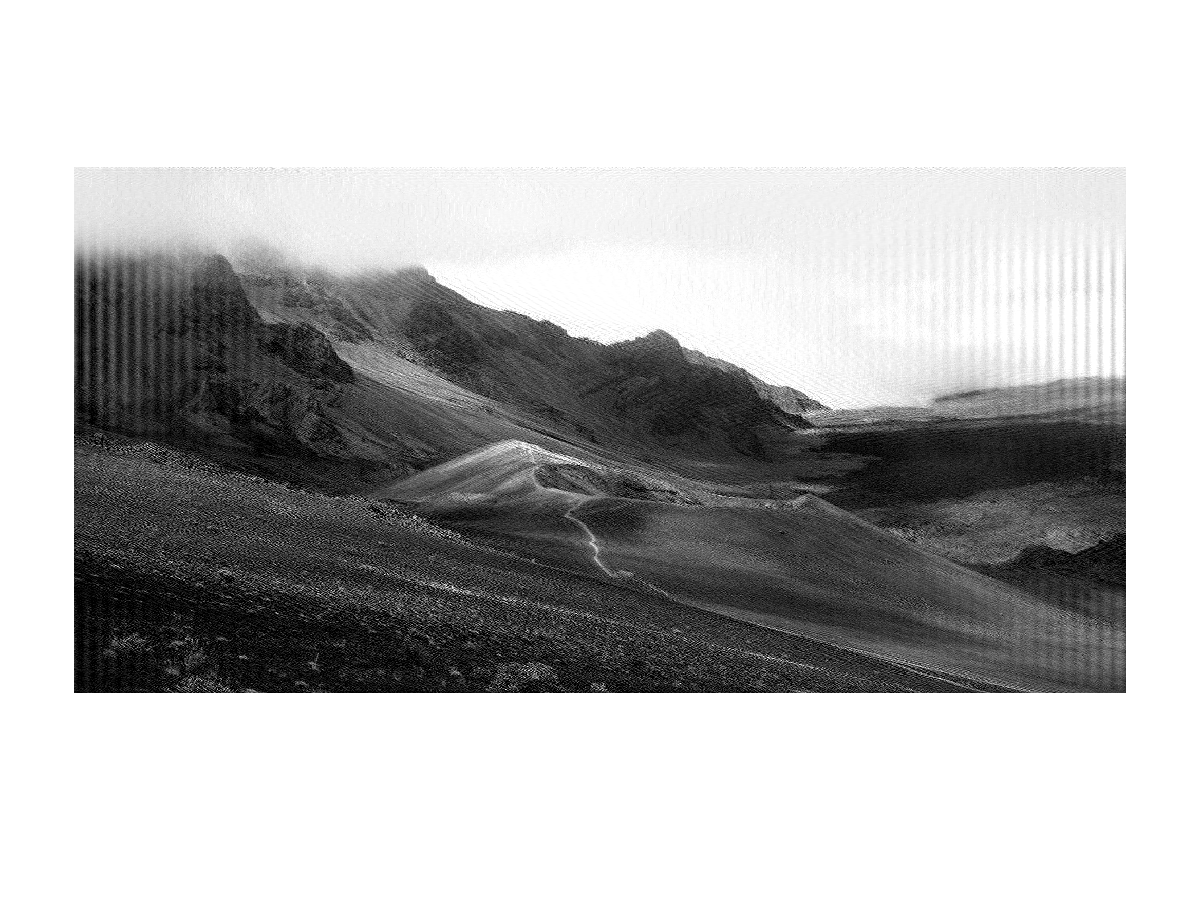
\includegraphics[width= \textwidth]{../Images/SagarShortEstimation.png}
\vspace{-30pt}
\caption{Picture deblurred using only a $256\times 256$ centered crop of the picture. }
\label{fig:SagarShort}
\end{subfigure}
~
\begin{subfigure}{0.4\textwidth}
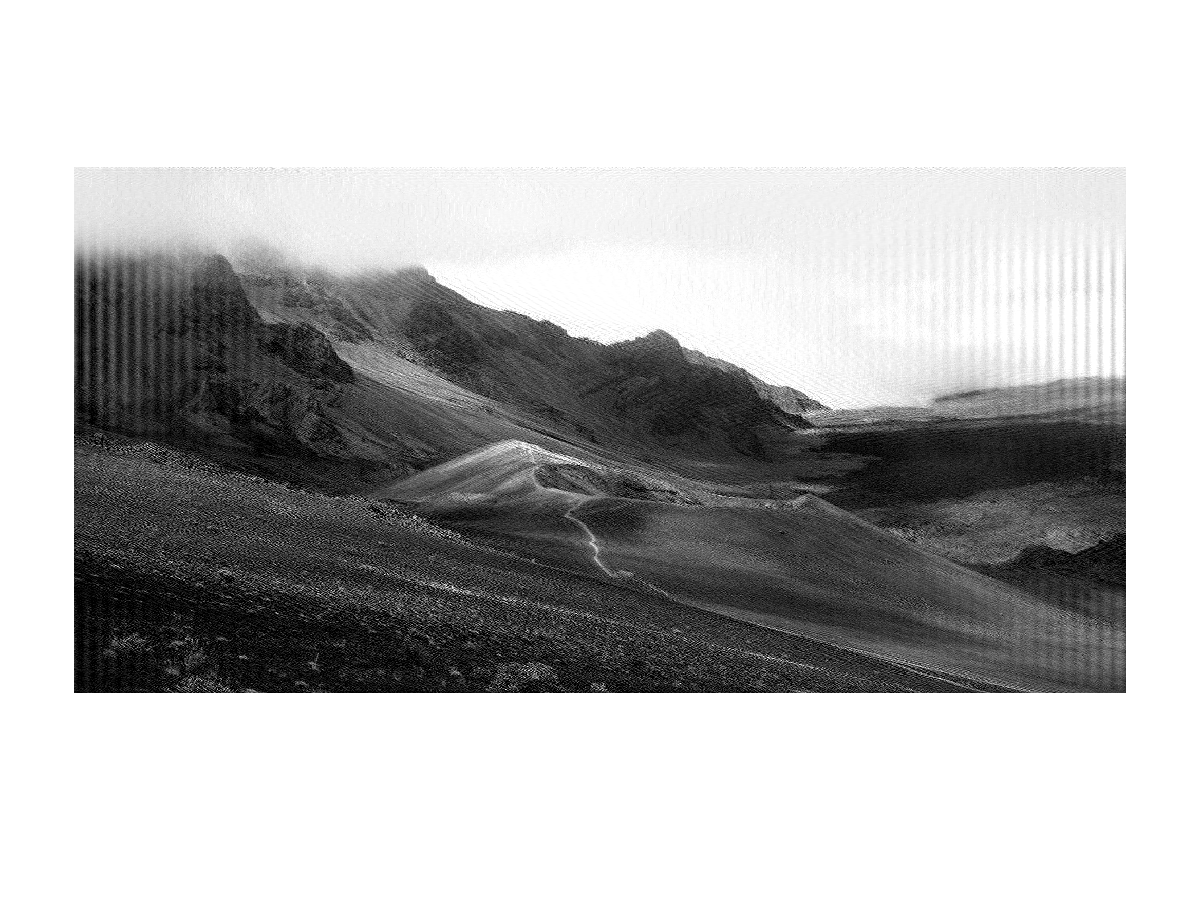
\includegraphics[{width= \textwidth}]{../Images/SagarLongEstimation.png}
\vspace{-30pt}
\caption{Picture deblurred using the whole image.}
\label{fig:SagarLong}
\end{subfigure}
\caption{Different matrix's size for the PSF estimation.}
\end{figure}

Another change is the image's resizing before the deconvolution. The goal is to reduce the number of pixels and so reduce the size of the matrix and the number of iterations needed in our loops.  However this resizing presents some challenges due to artifacts which can appear during the process.

\todo{Merge from here}
The main artifacts which can occur depending on the algorithm are the moiré pattern and picture's softening.  
The first one, the moiré pattern is due to an insufficient number of pixels to replicate a specific pattern. We reduce the resolution so we have to cut off the high frequencies from the original image in order to have only the supported frequencies in the resized one. If we do not so, some Moiré pattern could appear.  However when a picture is blurred, as the pixels of the pattern are spread, these artifacts are less problematic. The figure \ref{fig:bricksOriginal} is processed in two different ways. The first one is a resized version using the Nearest Neighbor algorithm, figure \ref{fig:bricksCompressed}, the second one is an artificially blurred version then resized and deblurred using the same resizing algorithm as before, figure \ref{fig:bricksDeblurred}. On the one hand, there is a strong moiré pattern on the figure \ref{fig:bricksCompressed}. On the other hand the deblurred picture \ref{fig:bricksDeblurred} has still a bit of Moiré, but the result is much better than the other picture. 
The second artifact, the picture's softening, is due to image processing which try to reduce the moiré pattern. Indeed the algorithm filter out a wider range of high frequency and so the picture is smoothed.  

So, as we have to deal with blurred image and want the sharpest result possible, we can reasonably use resizing algorithms which allow the best sharpness even if they produce Moiré pattern. 

\todo{To here}
The main artifacts which can occur depending on the algorithm are the moiré pattern and picture's softening.
The first one, the moiré pattern is due to an insufficient number of pixels to replicate a specific pattern. However when a picture is blurred, as the pixels of the pattern are spread, these artifact is less problematic. The figure \ref{fig:bricksOriginal} is processed in two different ways. The first one is a resizing using the Nearest Neighbor algorithm, figure \ref{fig:bricksCompressed}, the second one is a artificial blur then a resizing and a deblur using the same resizing algorithm as before, figure \ref{fig:bricksDeblurred}. On the one hand, there is a strong moiré pattern on the figure \ref{fig:bricksCompressed}. On the other hand the deblurred picture \ref{fig:bricksDeblurred} has still a bit of Moiré, but the result is much better than the other picture.
The second artifact, the picture's softening, is due to image processing which try to reduce the moiré artifact.

So, as we have to deal with blurred image and want the sharpest result possible, we can reasonably use resizing algorithm which allow the best sharpness even if they produce Moiré pattern.
\todo{With here}

\begin{figure}[h]
\centering
\begin{subfigure}{0.3\textwidth}
% The image is missing
%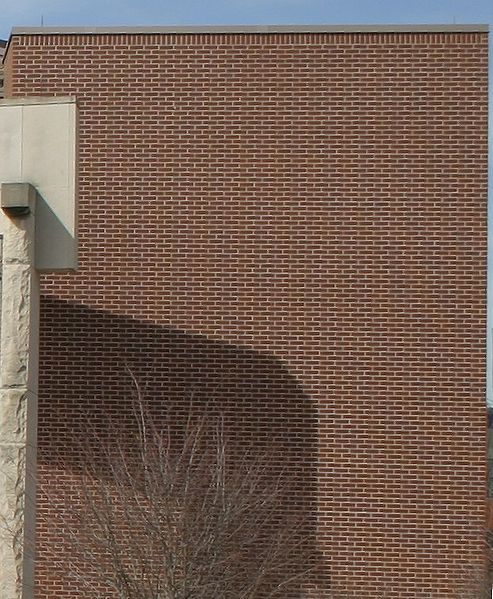
\includegraphics[width= \textwidth]{../Images/bricks.jpg}
\vspace{-30pt}
\caption{Original picture.}
\label{fig:bricksOriginal}
\end{subfigure}
~
\begin{subfigure}{0.4\textwidth}
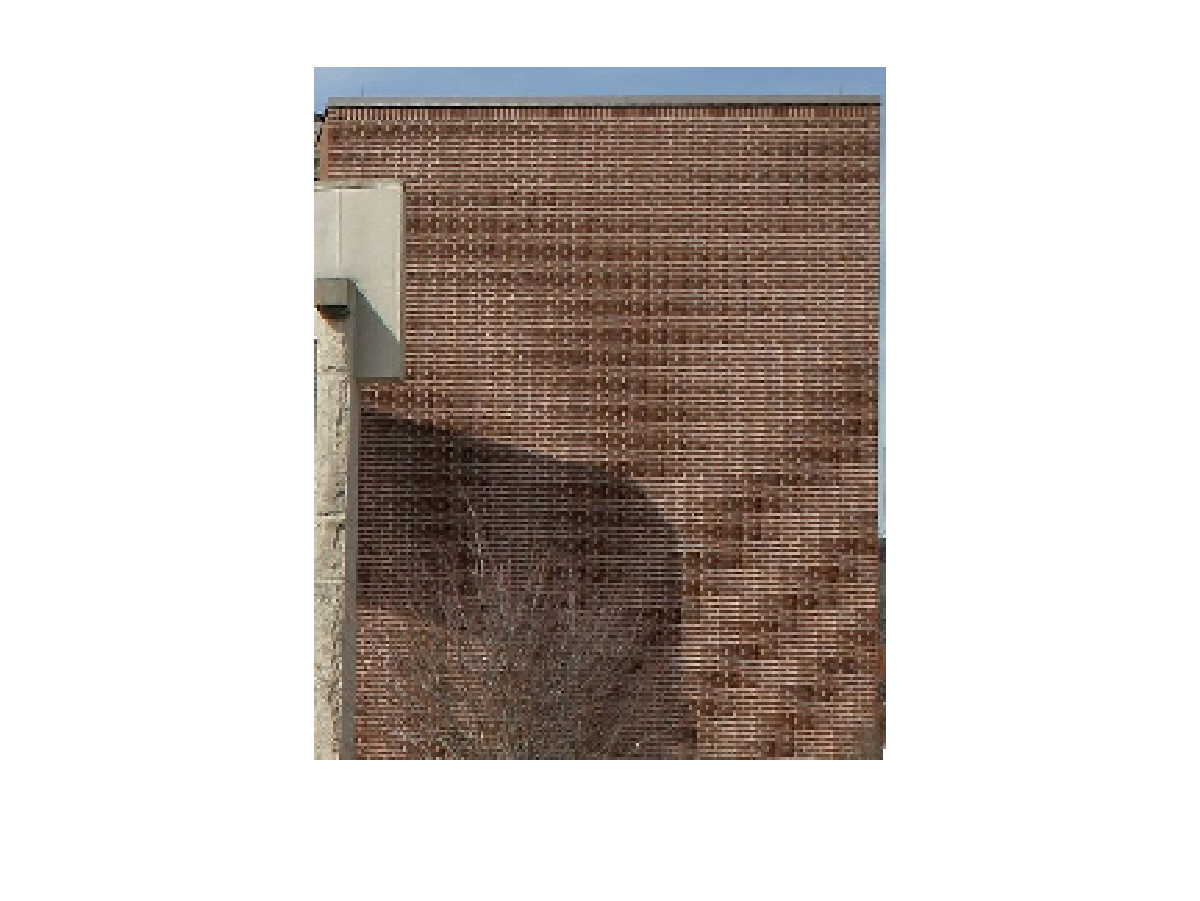
\includegraphics[width= \textwidth]{../Images/bricksCompressed.png}
\vspace{-30pt}
\caption{Picture resized using Nearest-Neighbor algorithm and no blur. }
\label{fig:bricksCompressed}
\end{subfigure}
~
\begin{subfigure}{0.4\textwidth}
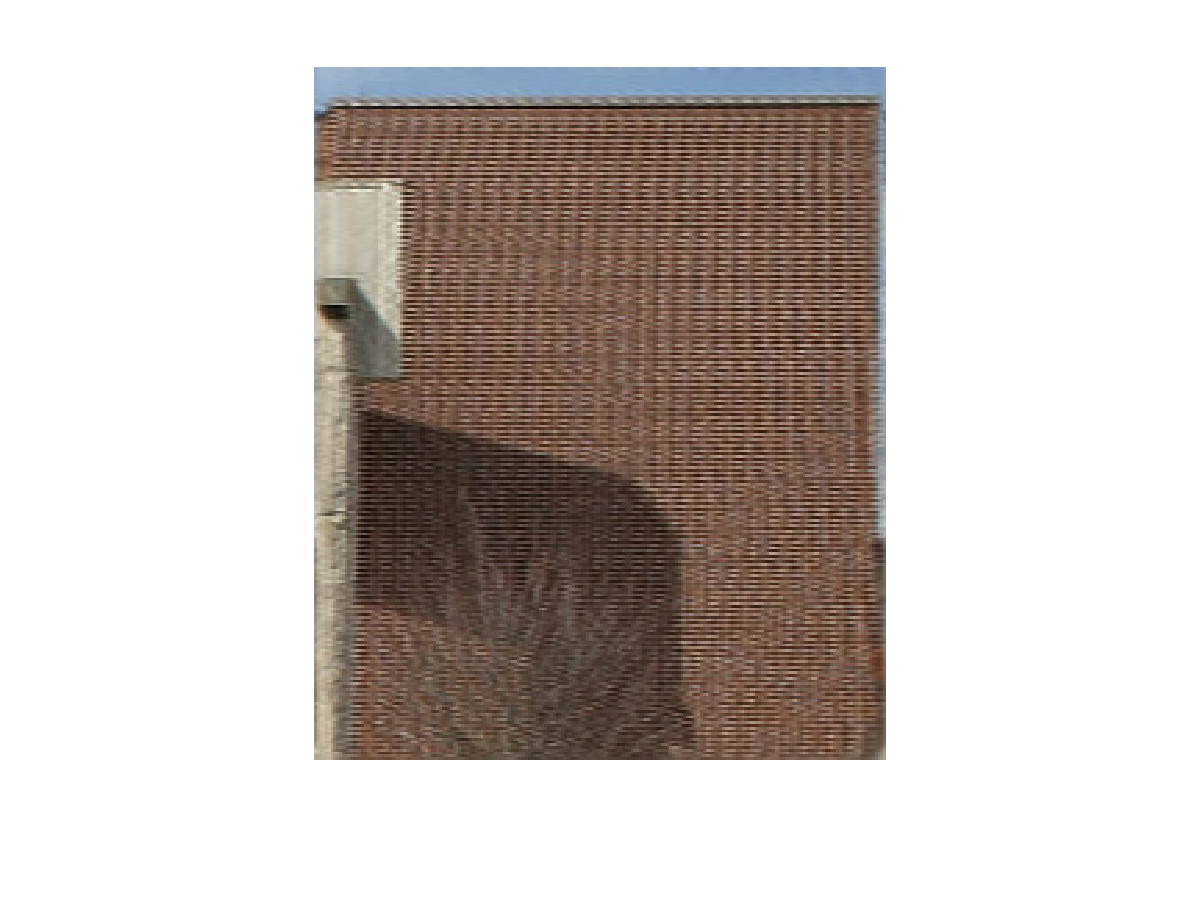
\includegraphics[{width= \textwidth}]{../Images/bricksDeblurred.png}
\vspace{-30pt}
\caption{Picture resized and deblurred using Nearest-Neighbor algorithm and Lucy-Richardson deconvolution.}
\label{fig:bricksDeblurred}
\end{subfigure}
\caption{Difference between resizing and resizing with blur.}
\end{figure}

There exist many different algorithms to resize pictures and some are better to preserve the sharpness. Among these, there is the Nearest-neighbor algorithm already used before. It operates in a easy way and is quick, around $0.002$ [s] to resize.  This algorithm selects points at constant distance depending on the resizing required and replaces all the other points by their nearest neighbor. %TODO source: wiki
 However the results are far from perfect.

So we decide to use another algorithm. The algorithm which is known to present %TODO source??
\todo{Merge from here}
the sharpest result without too much artifact is Lanczos. It is based on a sinc multiplied by a windowing function. The a-lobed Lanczos-windowed sinc function is defined as 
\[
Lanczos2(x) = 
\left\{  \begin{array}{cc}
\frac{\sin(\pi x )}{\pi x} \frac{\sin (\pi \frac{x}{a}) }{\pi \frac{x}{a}}, & |x| < a\\
0, & |x| \geq a
\end{array} \right. \]

\todo{To here}
the sharpest result is lanczos. It is based on a sinc multiplied by a windowing function. For example the two-lobed Lanczos-windowed sinc function is defined as
\begin{equation*}
Lanczos2(x) =
\begin{cases}
\frac{\sin(\pi x )}{\pi x} \frac{\sin (\pi \frac{x}{2}) }{\pi \frac{x}{2}}, & |x| < 2\\
0, & |x| \geq 2
\end{cases}
\end{equation*}
\todo{With here}
%TODO source : ResamplingFilters.pdf
%TODO perhaps add the explenation of the filter ? 
The first sinc creates a box in the frequency domain which cut off the high frequencies. The inequality gives a finite support to this sinc. However it represents a convolution by a sinc in frequency which generates some artifacts. To decrease these, we have to convolve the first box by a smaller one in order to smooth its sides, so we multiply by another sinc in spatial domain. 
%Source http://stackoverflow.com/questions/1854146/what-is-the-idea-behind-scaling-an-image-using-lanczos/1858632#1858632?newreg=cfaa7e1ec4044b47a551470a46df8b17
There is two lobed Lanczos-windowed sinc function, three lobed Lanczos-windowed sinc function, four lobed etc. Because or goal is to have a fast algorithm, we prefer to keep $Lanczos2$ (average computation time :  0.012 [s]) instead of $Lanczos3$ (average computation time : 0.016 [s]). 


\begin{figure}
\centering
%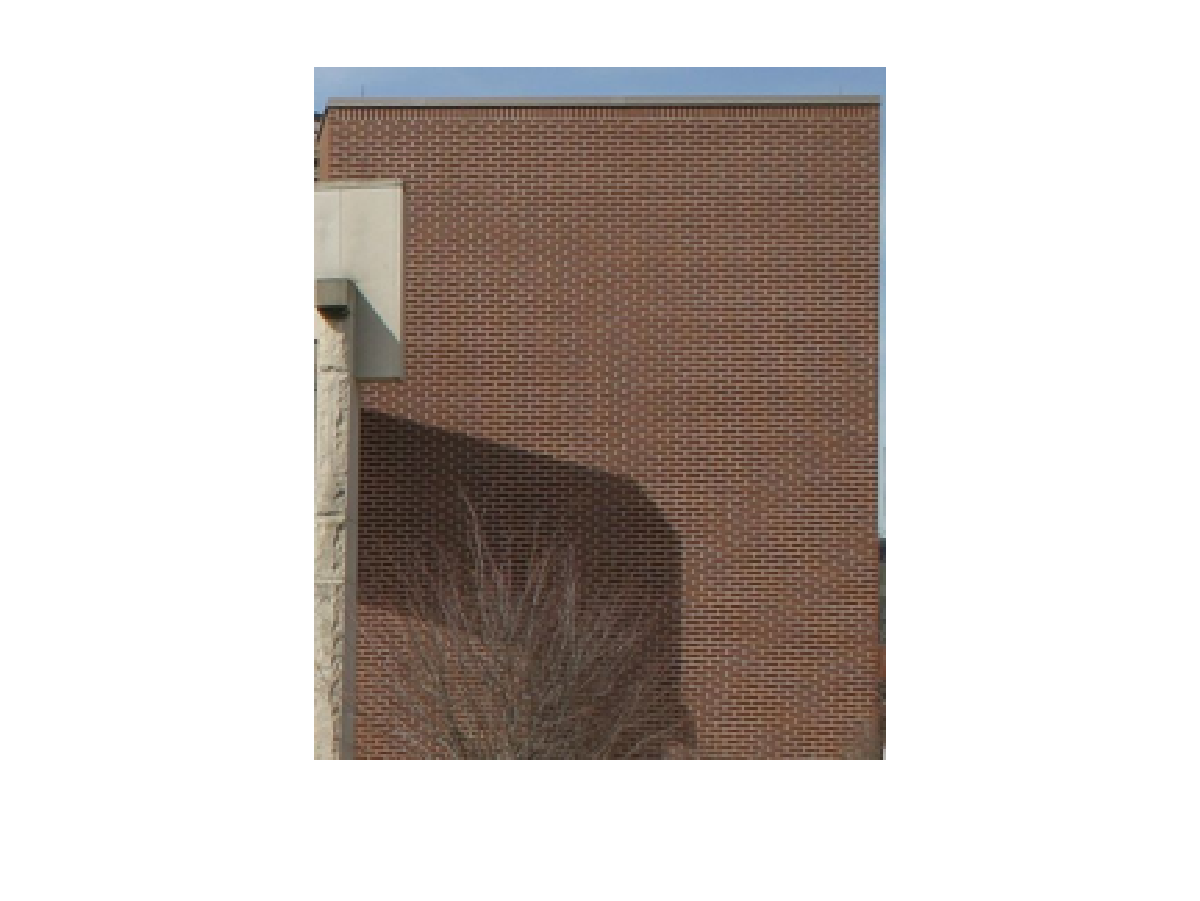
\includegraphics[width=\textwidth]{../Images/bricksLanczos.png}
\missingfigure{Tu l'as pas push...}
\label{fig:bricksLanczos}
\caption{Picture processed in the same way as \ref{fig:bricksDeblurred} }
\end{figure}
%Notre critère supplémentaire est une attention particulière au temps de calcul nécessaire pour le défloutage. 
%Nous avons donc mis divers procédés en place pour réduire le temps de calcul 
%
%Comprimer l'image s'avère nécessaire dans certains cas pour ramener le temps de calcul dans des limites acceptables, et plus particulièrement pour notre item supplémentaire, le \textit{``real time''} (cf. section).
